\documentclass[14pt, a4paper]{extarticle}
\usepackage{GOST}
\usepackage{array}
\usepackage{verbatim}
\usepackage[detect-all]{siunitx}
\usepackage{amsmath}
\usepackage{amssymb}
\usepackage[utf8]{inputenc}
\usepackage{hyperref}

\usepackage{ifthen}


\usepackage{tempora}



\makeatletter
\renewcommand\@biblabel[1]{#1.}
\makeatother

% Для листинга кода:
\usepackage{listings}
\lstset{ %
	language=c++,                 % выбор языка для подсветки (здесь это С)
	basicstyle=\small\sffamily, % размер и начертание шрифта для подсветки кода
	numbers=left,               % где поставить нумерацию строк (слева\справа)
	numberstyle=\tiny,           % размер шрифта для номеров строк
	stepnumber=1,                   % размер шага между двумя номерами строк
	numbersep=5pt,                % как далеко отстоят номера строк от подсвечиваемого кода
	showspaces=false,            % показывать или нет пробелы специальными отступами
	showstringspaces=false,      % показывать или нет пробелы в строках
	showtabs=false,             % показывать или нет табуляцию в строках
	frame=single,              % рисовать рамку вокруг кода
	tabsize=2,                 % размер табуляции по умолчанию равен 2 пробелам
	captionpos=t,              % позиция заголовка вверху [t] или внизу [b] 
	breaklines=true,           % автоматически переносить строки (да\нет)
	breakatwhitespace=false, % переносить строки только если есть пробел
	escapeinside={\#*}{*)}   % если нужно добавить комментарии в коде
}


%для графиков
\usepackage{pgfplots}
\usepackage{filecontents}
\usetikzlibrary{datavisualization}
\usetikzlibrary{datavisualization.formats.functions}

\begin{document}
	
	\begin{table}[ht]
		\centering
		\begin{tabular}{|c|p{400pt}|} 
			\hline
			\begin{tabular}[c]{@{}c@{}} 
\includegraphics[scale=1]{baum.jpg} \\\end{tabular} &
			\footnotesize\begin{tabular}[c]{@{}c@{}}\textbf{Министерство~науки~и~высшего~образования~Российской~Федерации}\\\textbf{Федеральное~государственное~бюджетное~образовательное~учреждение}\\\textbf{~высшего~образования}\\\textbf{«Московский~государственный~технический~университет}\\\textbf{имени~Н.Э.~Баумана}\\\textbf{(национальный~исследовательский~университет)»}\\\textbf{(МГТУ~им.~Н.Э.~Баумана)}\\\end{tabular}  \\
			\hline
		\end{tabular}
	\end{table}
	\noindent\rule{\textwidth}{4pt}
	\noindent\rule[14pt]{\textwidth}{1pt}
	\hfill 
	\noindent
	\makebox{ФАКУЛЬТЕТ~}%
	\makebox[\textwidth][l]{\underline{~«Информатика и системы управления»~~~~~~~~~~~~~~~~~~~~~~~~~~~~~~~~~}}%
	\\
	\noindent
	\makebox{КАФЕДРА~}%
	\makebox[\textwidth][l]{\underline{~«Программное обеспечение ЭВМ и информационные технологии»~}}%
	\\
	
	\begin{center}
		\vspace{1.5cm}
		{\bf\huge Отчёт\par}
		{\bf\Large по лабораторной работе № 3\par}
		\vspace{0.7cm}
	\end{center}
	
	
	\noindent
	\makebox{\large{\bf Название:}~~~}
	\makebox[\textwidth][l]{\large\underline{Основы Linux~~~~~~~~~~~~~}}\\
	
	\noindent
	\makebox{\large{\bf Дисциплина:}~~~}
	\makebox[\textwidth][l]{\large\underline{~Операционные системы~~~~~~~~~~~~~~~~~~~~~~~~~~}}\\
	
	\vspace{1.5cm}
	\noindent
	\begin{tabular}{l c c c c c}
		Студент      & ~ИУ7-55Б~               & \hspace{2.5cm} & \hspace{2cm}                 & &  Д.В. 
		Сусликов \\\cline{2-2}\cline{4-4} \cline{6-6} 
		\hspace{3cm} & {\footnotesize(Группа)} &                & {\footnotesize(Подпись, дата)} & & {\footnotesize(И.О. Фамилия)}
	\end{tabular}
	
	\noindent
	\begin{tabular}{l c c c c}
		Преподаватель & \hspace{5cm}   & \hspace{2cm}                 & & ~~~~~~Н.Ю. Рязанова~~~~~~\\\cline{3-3} \cline{5-5} 
		\hspace{3cm}  &                & {\footnotesize(Подпись, дата)} & & {\footnotesize(И.О. Фамилия)}
	\end{tabular}
	
	\vspace{0.6cm}
	\begin{center}	
		\vfill
		\large \textit {Москва, 2020}
	\end{center}
	
	\thispagestyle {empty}
	\pagebreak
	
	% СОДЕРЖАНИЕ 
	\clearpage
	\tableofcontents
	
	
	% ВВЕДЕНИЕ
	\clearpage
	\section{Задание 1}
	Изучение команд Shell.
	
	Задание:
	\begin{enumerate}
		\item используя команду mkdir cоздайте директорию имeнем своей группы. Например, mkdir iu7; перейдите в созданную директорию с помощью команды cd;
		\item создайте поддиректорию, например, используя свою фамилию;
		\item воспользоваться командой ls;
		\item воспользоваться командой ps.	
	\end{enumerate}
	
	На Рисунке 1 показано создание директории и поддиректории, вывод списка файлов, списка процессов:
	\begin{figure}[h!]
		\centering
		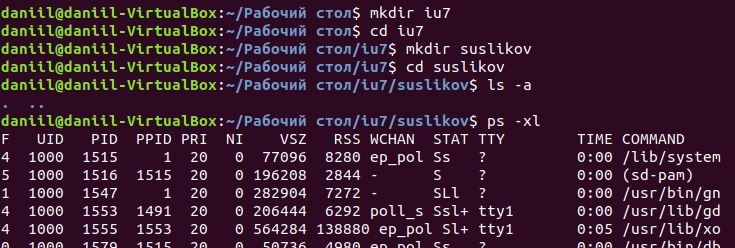
\includegraphics[scale=1]{source/1}
		\caption{Задание 1}
	\end{figure}
	
	\clearpage
	\section{Задание 2}
	Задание:
	\begin{enumerate}
		\item напишите программу, в которой создается дочерний процесс и организуйте как в предке, так и в
		потомке бесконечные циклы, в которых выводятся идентификаторы процессов с помощью системного
		вызова getpid();
		\item запустите программу и посмотрите идентификаторы созданных процессов: предка и потомка;
		\item для получения процесса зомби выполните следующие действия: a) удалите командой kill потомка и
		посмотрите с помощью команды ps его новый статус – Z; b) удалите предка;
		\item Для получения «осиротевшего» процесса запустите программу еще раз, но в этот раз удалите предка и посмотрите с помощью команды ps идентификатор предкка у продолжающего выполняться
		потомка – идентификатор предка будет изменен на 1, так как процесс был «усыновлен» процессом с
		идентификатором 1 процессом «открывшим» терминал в случае, если используется Unix BSD, или
		идентификатор процессов-посредников в случае, Linux Ubuntu.	
	\end{enumerate}
	
	В Листинге 1 представлена требуемая программа.\newline
	Листинг 1 - программа.
	\begin{lstlisting}		
		#include <stdio.h>
		#include <unistd.h>
		
		int main()
		{
			int childpid;
			if ((childpid = fork())== -1)
			{
				perror("Can't fork.\n");
				return 1;
			}
			else if (childpid == 0)
			{
				while (1) printf(" %d ", getpid());
				return 0;
			}
			else
			{
				while(1) printf(" %d ",getpid());
				return 0;
			}
		}
	\end{lstlisting}


	Результат работы программы представлен на Рисунке 2.
	\begin{figure}[h]
		\centering
		
\includegraphics[scale=1]{source/2}
		\caption{Результат работы программы}
	\end{figure}
	
	На Рисунке 3 можно увидеть id потомка и предка.
	\begin{figure}[h]
		\centering
		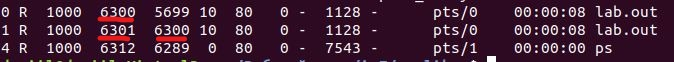
\includegraphics[scale=1]{source/3v2}
		\caption{Результат команды ps -xl}
	\end{figure}
	
	\newpage
	Создание зомби. \newline
	Получение процесса зомби показано на Рисунке 4.
	\begin{figure}[h]
		\centering
		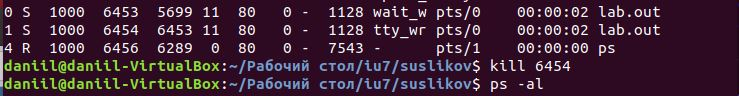
\includegraphics[scale=1]{source/41}
		\caption{Получение процесса зомби}
	\end{figure}

	Результат команды kill потомка изображен на Рисунке 5.
	\begin{figure}[h]
		\centering
		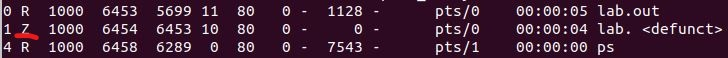
\includegraphics[scale=1]{source/4v2}
		\caption{Результат команды kill потомка}
	\end{figure}
	
	Создание сироты. \newline
	Получение процесса сироты показано на Рисунке 6.
	\begin{figure}[h!]
		\centering
		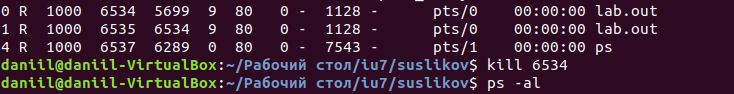
\includegraphics[scale=1]{source/5}
		\caption{Получение процесса сироты}
	\end{figure}

	Результат (усыновление) продемонстрирован на Рисунке 7.
	\begin{figure}[h!]
		\centering
		
\includegraphics[scale=1]{source/52v2}
		\caption{Результат создания процесса сироты}
	\end{figure}
	 
	 \clearpage
	 \section{Задание 3}
	 Продемонстрировать работу pipe. \newline
	 Создание pipe и запись в него строки показано на Рисунке 8.
	 \begin{figure}[h!]
	 	\centering
	 	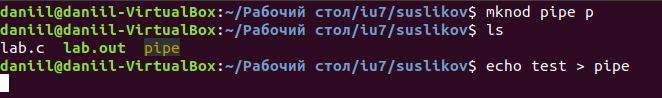
\includegraphics[scale=1]{source/6}
	 	\caption{Создание pipe и запись в него строки}
	 \end{figure}
	
	На Рисунке 9 показано чтение из pipe.
	\begin{figure}[h!]
		\centering
		
\includegraphics[scale=1]{source/7}
		\caption{Создание pipe и запись в него строки}
	\end{figure}

	\clearpage
	\section{Задание 4}
	Создать hardlink и softlink.\newline
	Создание hardlink показано на Рисунке 10.
	\begin{figure}[h]
		\centering
		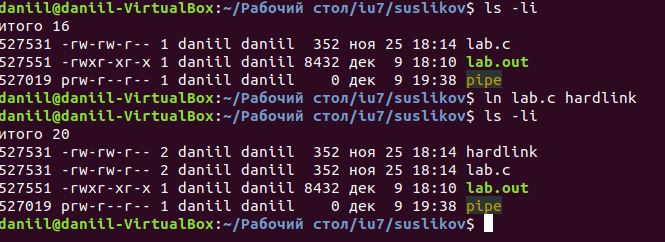
\includegraphics[scale=1]{source/8}
		\caption{Создание hardlink}
	\end{figure}

	Создание softlink изображено на Рисунке 11.
	\begin{figure}[h]
		\centering
		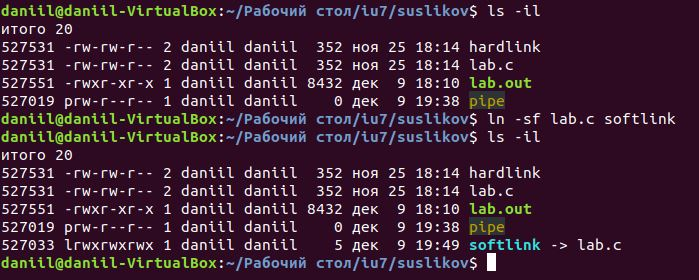
\includegraphics[scale=1]{source/9}
		\caption{Создание softlink }
	\end{figure}

\end{document}